\section{Results}

\subsection{Overview}

The results answer five questions about credible recommendation under partial
observation. RQ1 asks whether verifier and claim-boundary checks prevent
leakage-prone or claim-unsafe evidence from supporting recommendations. RQ2
tests whether the selection logic can recover known observation and delay
labels in controlled structured time-series tasks. RQ3 evaluates whether
candidate orderings reach useful candidates under fixed budgets in synthetic
execution, frozen replay, and bounded real-data execution. RQ4 compares real
LLM provider families only as constrained structured proposers. RQ5 returns to
the FluSurv-NET case study and asks what the evidence supports about
age-specific, objective-specific model recommendation.

The main text reports only the aggregate metrics needed to answer these RQs.
Full provider benchmark tables, detailed candidate-budget replay rows,
bounded-execution diagnostics, the discovery-ablation matrix, the numerical
failure audit, and the multi-season robustness tables are treated as
supplementary evidence in the compact reports and artifact CSVs.

\subsection{RQ1: Verifier and claim-boundary auditing}

The offline verifier rejects the full negative set of malformed or unsafe
records, giving rejection rate \num{1.0}. Rejected cases include missing
required fields, duplicate candidate identifiers, absolute artifact paths,
selection evidence that incorrectly includes held-out test metrics,
numerically flagged rows used as positive evidence, and invalid observation or
delay labels. The same audit labels the frozen evidence as supporting no
single global winner, group-specific signals, simple-baseline competitiveness,
post-hoc comparisons not being selection evidence, and flagged numerical rows
being descriptive only.

The claim-boundary auditor rejects global-winner, state-of-the-art,
flagged-row-positive, autonomous-science, and real-world mechanism-recovery
claims. Held-out test metrics appear only as post-hoc descriptive fields after
selection. This first result is a software and evidence-provenance result: it
does not improve forecasts by itself, but it determines which downstream
recommendations are admissible.

The optional API-assisted proposal smoke test is consistent with this
boundary. It produced 10 allowlisted candidate records with verifier validity
\num{1.0}, duplicate rate \num{0.0}, four model-family categories, two
observation-label categories, and no claim-safety violations. The smoke test
is proposal-quality evidence only: API outputs are parsed as JSON,
allowlisted, and verifier-checked before use, and no API output generates or
executes model code.

\subsection{RQ2: Synthetic structured recovery}

The expanded synthetic structured recovery sweep evaluates controlled
structured time-series tasks with known direct, lagged, mixture, and proxy
observation labels. It uses 100 seeds, five noise levels, five candidate
budgets, and \num{75000} policy-condition rows before aggregation. These tasks
are generic software validation for observation-label and delay-label
selection logic; they are not real-world mechanism-discovery evidence.

In the full sweep, \texttt{pareto\_epsilon} recovers the observation label at
rate \num{0.7429}, the delay label at rate \num{0.7470}, and reaches
top-epsilon hit rate \num{0.8504}. The random-label baseline has
observation-label recovery \num{0.2597}, while the no-observation-label
baseline has observation-label recovery \num{0.2000}. At noise level
\num{0.10}, \texttt{pareto\_epsilon} observation-label recovery remains
\num{0.6800}. Its budget curve rises from \num{0.5720} at budget \num{3} to
\num{0.8356} at budget \num{10} and remains at that level for larger budgets.

\begin{figure}[H]
\centering
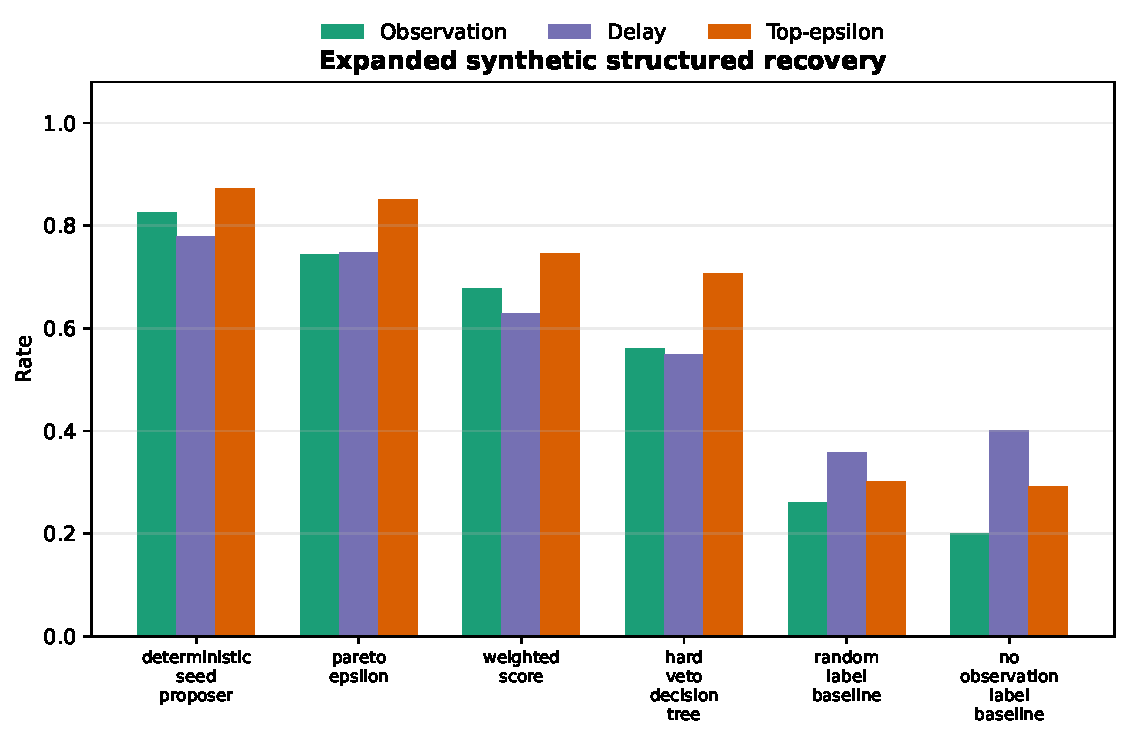
\includegraphics[width=0.92\textwidth]{figures/fig_synthetic_recovery_full_policy_comparison.pdf}
\caption{Expanded synthetic structured recovery over generic time-series toy
tasks. The figure summarizes observation-label, delay-label, and top-epsilon
hit rates for deterministic selection policies and baselines. These tasks are
software validation for selection logic, not evidence of real-world mechanism
recovery.}
\label{fig:synthetic-recovery-full-policy}
\end{figure}

Pareto-epsilon and deterministic seed policies substantially outperform random
and observation-fixed baselines, but Pareto is not universally best. The
deterministic seed proposer has observation-label recovery \num{0.8257},
higher than \texttt{pareto\_epsilon} in this controlled sweep. The strongest
synthetic evidence is in \texttt{lagged\_signal\_1} and
\texttt{lagged\_signal\_2}, where policies that can choose lagged observation
labels outperform the no-observation-label baseline. Mixture and proxy tasks
remain harder.

\begin{figure}[H]
\centering
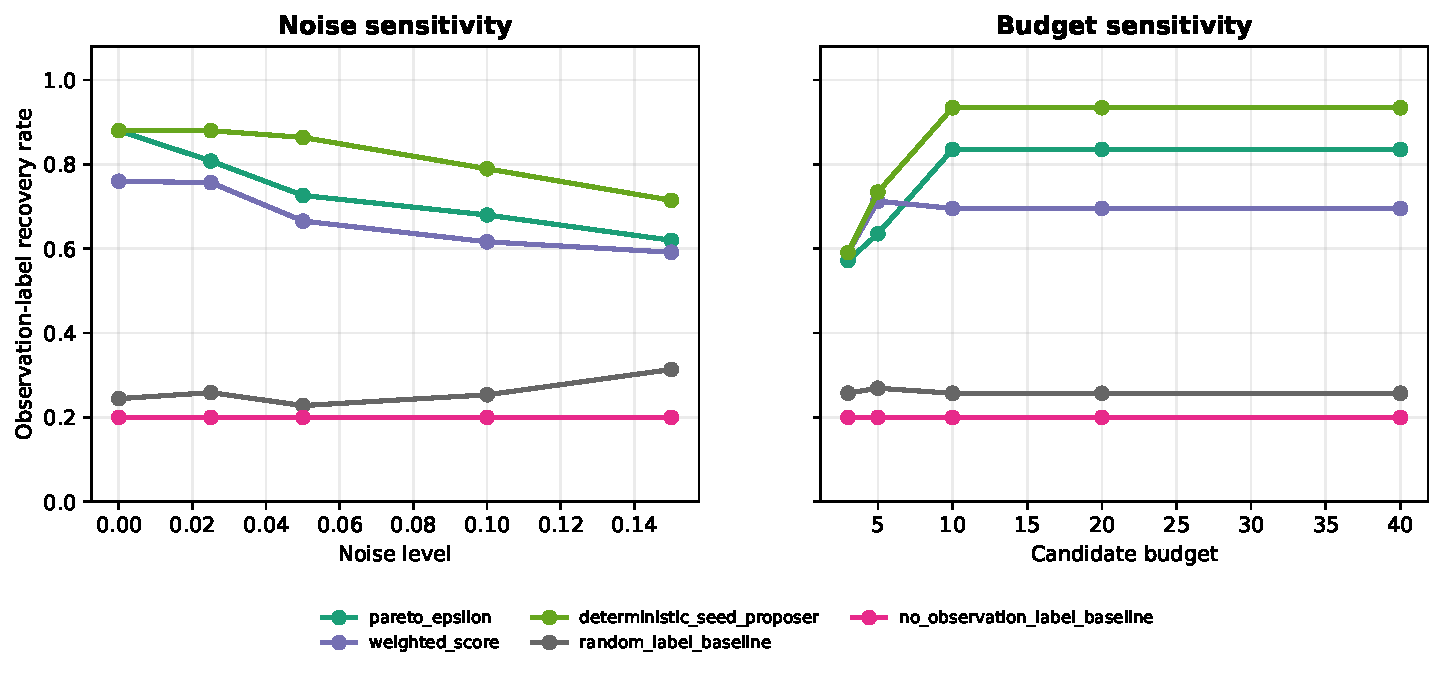
\includegraphics[width=\textwidth]{figures/fig_synthetic_recovery_full_noise_budget.pdf}
\caption{Noise and budget sensitivity in the expanded synthetic structured
recovery sweep. The curves show observation-label recovery under increasing
noise and candidate budget. This is a local software check over generic toy
tasks and is not used as a real-data forecasting-performance result.}
\label{fig:synthetic-recovery-full-noise-budget}
\end{figure}

\subsection{RQ3: Candidate-budget execution and bounded real-data execution}

Candidate-budget evaluation asks whether proposer orderings expose useful
candidates quickly. In synthetic execution, the mock API proposer has
observation-label recovery \num{0.9313}, delay-label recovery \num{0.9190},
and top-epsilon hit rate \num{1.0000}. The failure-guided proposer is similar
(\num{0.9233}, \num{0.9113}, and \num{1.0000}). The deterministic seed
proposer reaches \num{0.7863} observation recovery, \num{0.7278} delay
recovery, and \num{0.8453} top-epsilon hit rate; the random candidate proposer
is competitive at \num{0.8208}, \num{0.7943}, and \num{0.9045}. The
no-observation-label baseline remains much weaker, with observation recovery
\num{0.2000}, delay recovery \num{0.4000}, and top-epsilon hit rate
\num{0.3210}.

\begin{figure}[H]
\centering
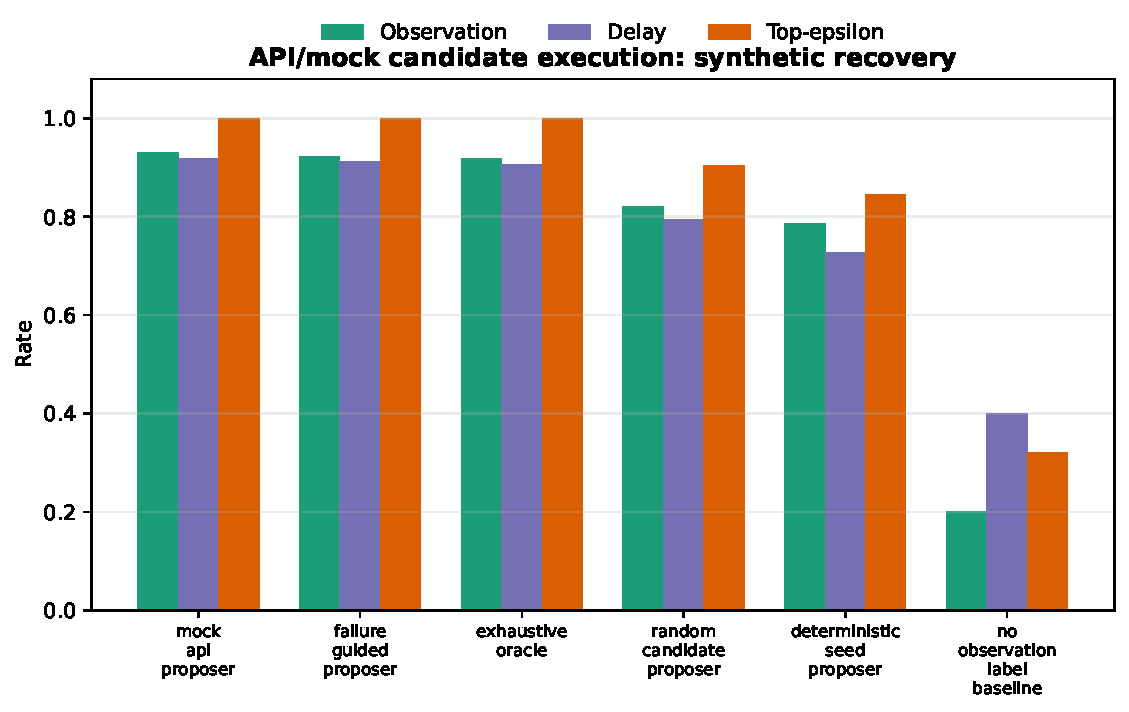
\includegraphics[width=0.92\textwidth]{figures/fig_api_synthetic_recovery_comparison.pdf}
\caption{Candidate execution over generic structured time-series toy tasks.
The mock API proposer and failure-guided proposer reach high label recovery
and top-epsilon rates under fixed budgets, while the observation-fixed
baseline remains weaker. This supports proposal-ordering and budget-efficiency
claims only.}
\label{fig:api-synthetic-recovery-comparison}
\end{figure}

Frozen real-data replay uses compact summary rows without refitting models.
In this replay, the mock API proposer reaches top-epsilon rate \num{1.0000}
with mean rolling score \num{0.0851}. The oracle ranking also has
top-epsilon rate \num{1.0000}, with mean rolling score \num{0.0830}. The
random candidate proposer reaches \num{0.8125} and \num{0.0925}; the
deterministic seed proposer reaches \num{0.7500} and \num{0.0949}. The prompt
audit has 46 rows and all pass; held-out test MAE is post-hoc descriptive
only.

\begin{figure}[H]
\centering
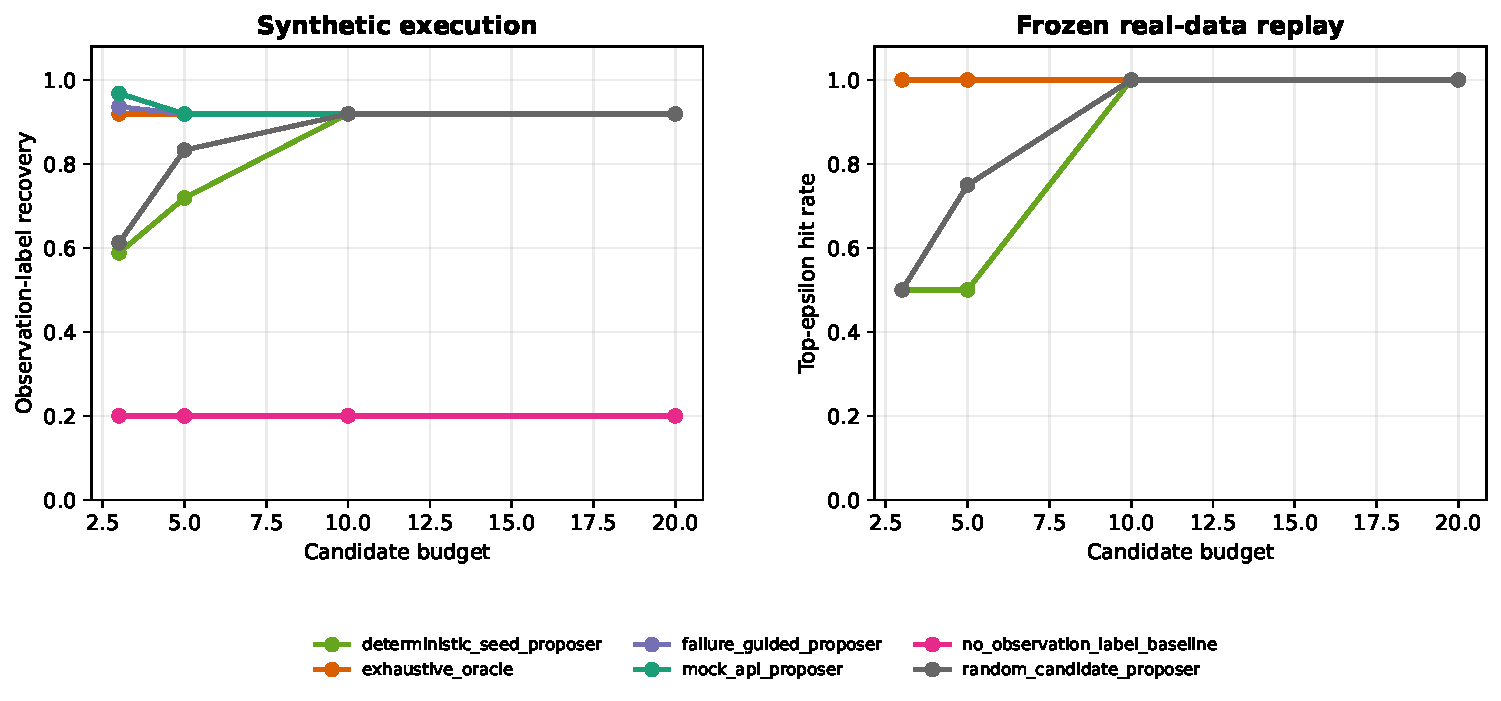
\includegraphics[width=\textwidth]{figures/fig_api_candidate_execution_budget.pdf}
\caption{Budget curves for synthetic execution and frozen real-data replay.
The real-data replay layer uses existing compact summary rows and performs no
model refitting. Random ordering is competitive in some settings, so the
supported claim is reliability and candidate-budget efficiency under the
verifier, not universal dominance.}
\label{fig:api-candidate-execution-budget}
\end{figure}

The bounded real-data execution layer executes allowlisted candidate models on
\texttt{0-4 yr}, \texttt{18-49 yr}, \texttt{Overall}, and \texttt{>=65 yr}
using reduced fitting and search budgets. It required 32 unique real-data
model executions. The deterministic seed proposer, failure-guided proposer,
mock API proposer, and oracle reference each reach top-epsilon hit rate
\num{1.00}; the random proposer reaches \num{0.75}. Mean rolling scores are
\num{0.0978} for deterministic seed, \num{0.0966} for failure-guided,
\num{0.0978} for mock API, \num{0.0978} for oracle reference, and
\num{0.1152} for random ordering. The no-leakage audit contains 52 rows and
all pass; test metrics remain post-hoc descriptive only.

\begin{figure}[H]
\centering
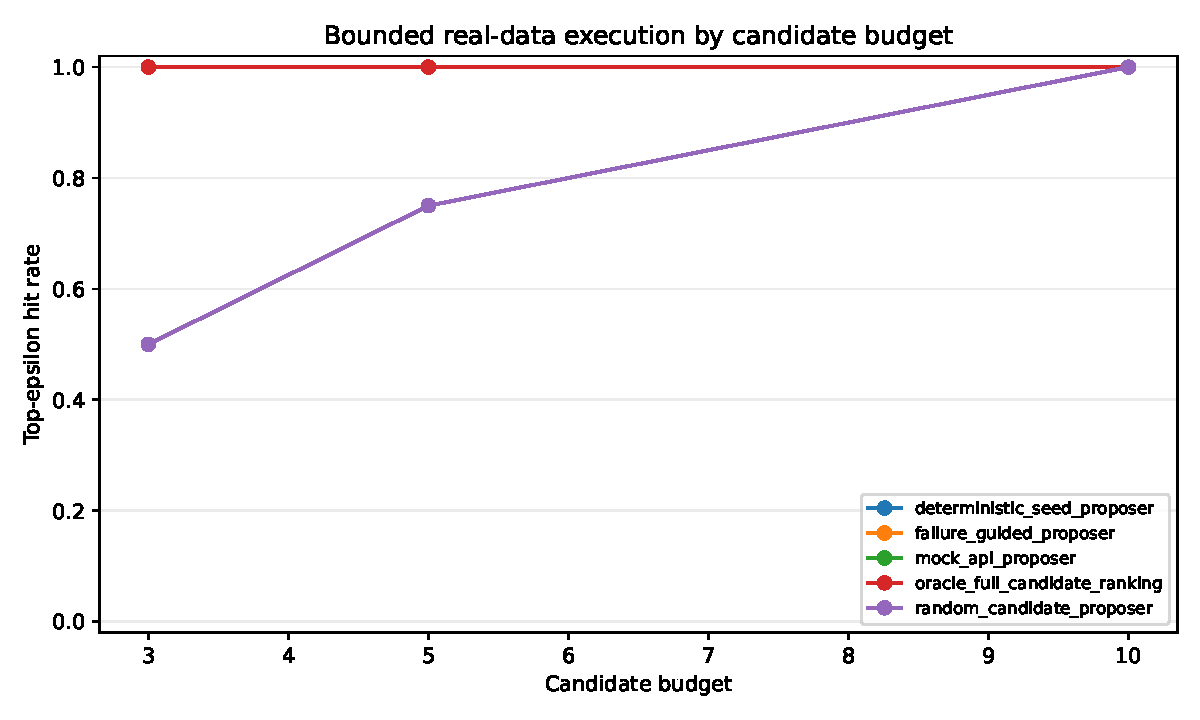
\includegraphics[width=\textwidth]{figures/fig_bounded_real_execution_budget.pdf}
\caption{Bounded real-data candidate execution under fixed candidate budgets.
Candidate ordering is evaluated after executing only allowlisted repository
models. The figure summarizes budget-efficiency evidence; it is not an
operational forecasting benchmark and does not support a state-of-the-art
claim.}
\label{fig:bounded-real-execution-budget}
\end{figure}

\subsection{RQ4: Cross-provider constrained proposer benchmark}

The cross-provider benchmark evaluates OpenAI/GPT, Anthropic/Claude,
Google/Gemini, and DeepSeek as structured candidate proposers under the same
prompt-task protocol, allowlist, verifier, and no-leakage audit. All four
providers enter the comparison after Gemini structured-output integration
hardening. Table~\ref{tab:provider-stage9} reports schema parse success,
verifier-valid proposal rate, and frozen replay top-epsilon hit rate. These
are proposal-quality and replay budget-efficiency metrics, not
forecasting-performance results.

\begin{table}[H]
\centering
\small
\caption{Cross-provider structured proposer results. All provider outputs are
JSON or structured-output parsed, allowlisted, verifier-checked, and audited
before replay. Top-epsilon hit is computed in frozen replay over compact
summaries.}
\label{tab:provider-stage9}
\begin{tabular}{lccc}
\toprule
Provider and mode & Schema parse & Valid proposals & Top-epsilon hit \\
\midrule
OpenAI iterative & \num{1.0000} & \num{0.9136} & \num{0.7778} \\
OpenAI single-shot & \num{1.0000} & \num{1.0000} & \num{0.8333} \\
Claude iterative & \num{1.0000} & \num{0.7901} & \num{0.7407} \\
Claude single-shot & \num{1.0000} & \num{0.8951} & \num{0.8333} \\
DeepSeek iterative & \num{1.0000} & \num{0.8519} & \num{0.8333} \\
DeepSeek single-shot & \num{1.0000} & \num{1.0000} & \num{0.9444} \\
Gemini iterative & \num{1.0000} & \num{0.7716} & \num{0.7778} \\
Gemini single-shot & \num{1.0000} & \num{0.9938} & \num{0.8333} \\
\midrule
Deterministic seed & \num{1.0000} & \num{1.0000} & \num{0.7778} \\
Failure-guided & \num{1.0000} & \num{1.0000} & \num{0.8333} \\
Random & \num{1.0000} & \num{1.0000} & \num{0.7222} \\
Oracle reference & \num{1.0000} & \num{1.0000} & \num{1.0000} \\
\bottomrule
\end{tabular}
\end{table}

The stabilized four-provider run shows that the same constrained protocol can
compare provider families without giving any provider access to held-out test
evidence or executable model-code pathways. Single-shot modes often match or
outperform iterative modes in this bounded allowlist setting: DeepSeek
single-shot reaches top-epsilon hit \num{0.9444}, while OpenAI, Claude, and
Gemini single-shot each reach \num{0.8333}. Iterative feedback is therefore a
constrained refinement protocol, but it is not automatically superior when the
candidate space is small and explicit. Failure-guided deterministic ordering
remains competitive at \num{0.8333}, random reaches \num{0.7222}, and the
oracle reference is \num{1.0000}.

\begin{figure}[H]
\centering
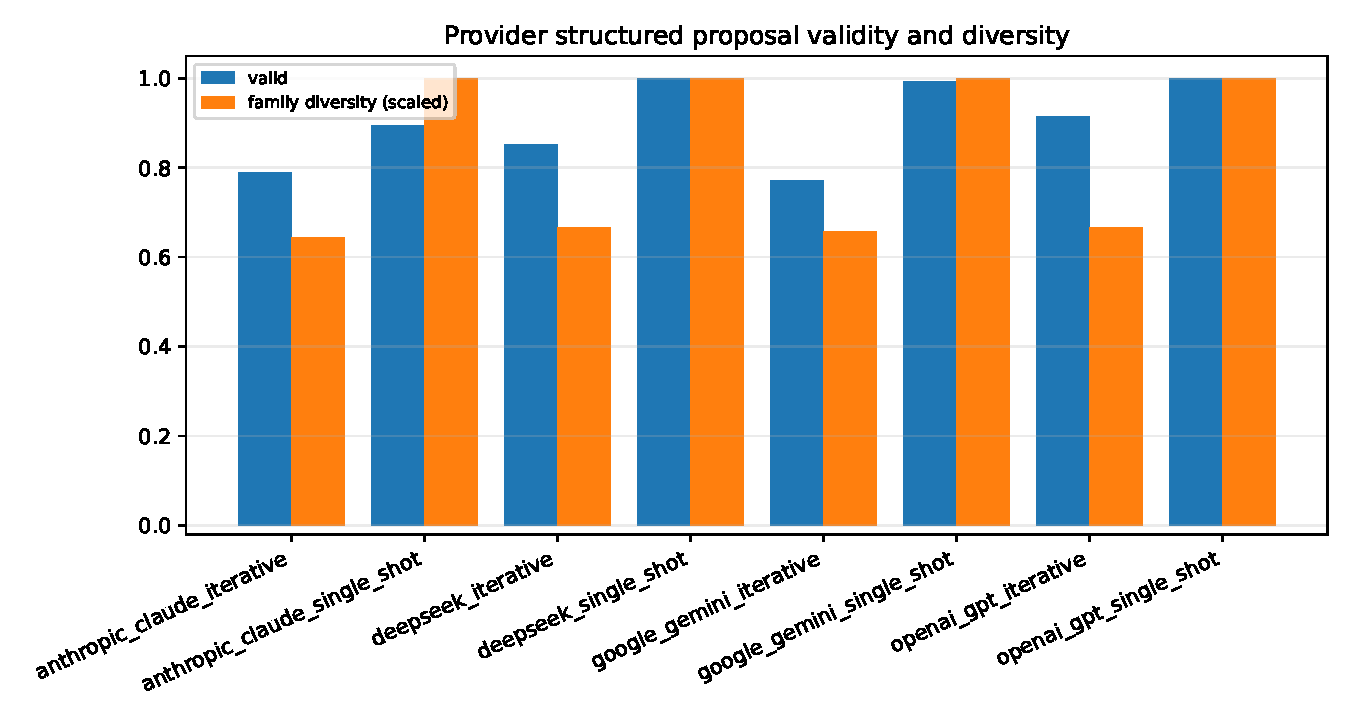
\includegraphics[width=\textwidth]{figures/fig_provider_validity_diversity.pdf}
\caption{Provider proposal validity and diversity under the shared allowlist,
verifier, and no-leakage protocol. The figure compares providers only as
structured candidate proposers; it is not a provider forecasting leaderboard.}
\label{fig:provider-validity-diversity}
\end{figure}

\begin{figure}[H]
\centering
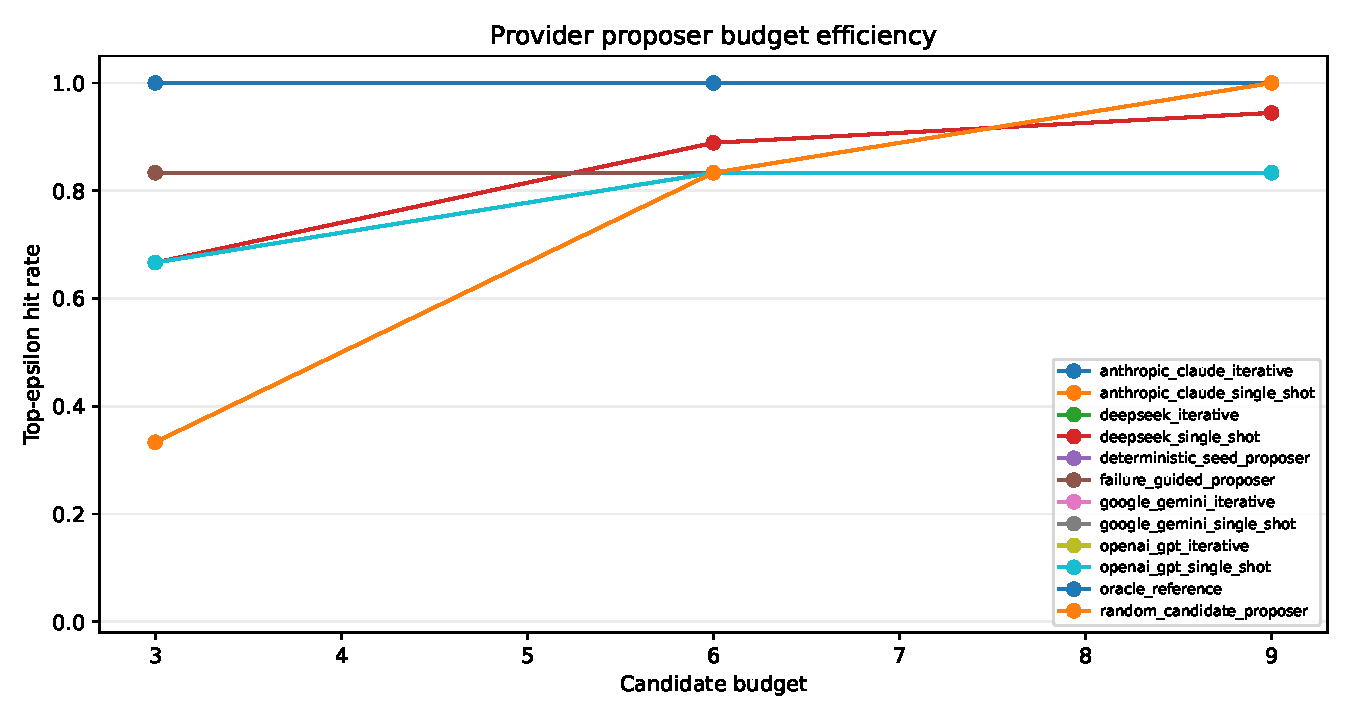
\includegraphics[width=\textwidth]{figures/fig_provider_budget_efficiency.pdf}
\caption{Frozen replay budget efficiency for provider and baseline proposal
orderings. The replay uses compact frozen summaries and supports
proposal-ordering evidence only, not new forecasting-performance claims.}
\label{fig:provider-budget-efficiency}
\end{figure}

\subsection{RQ5: FluSurv-NET case study and multi-season robustness}

The FluSurv-NET case study supports age-aware and objective-aware
recommendation rather than a single global winner. Table~\ref{tab:frozen-recommendations}
summarizes the frozen recommendation table derived from
\texttt{artifacts\_discovery\_ablation/paper\_recommendation\_table.csv}.

\begin{figure}[H]
\centering
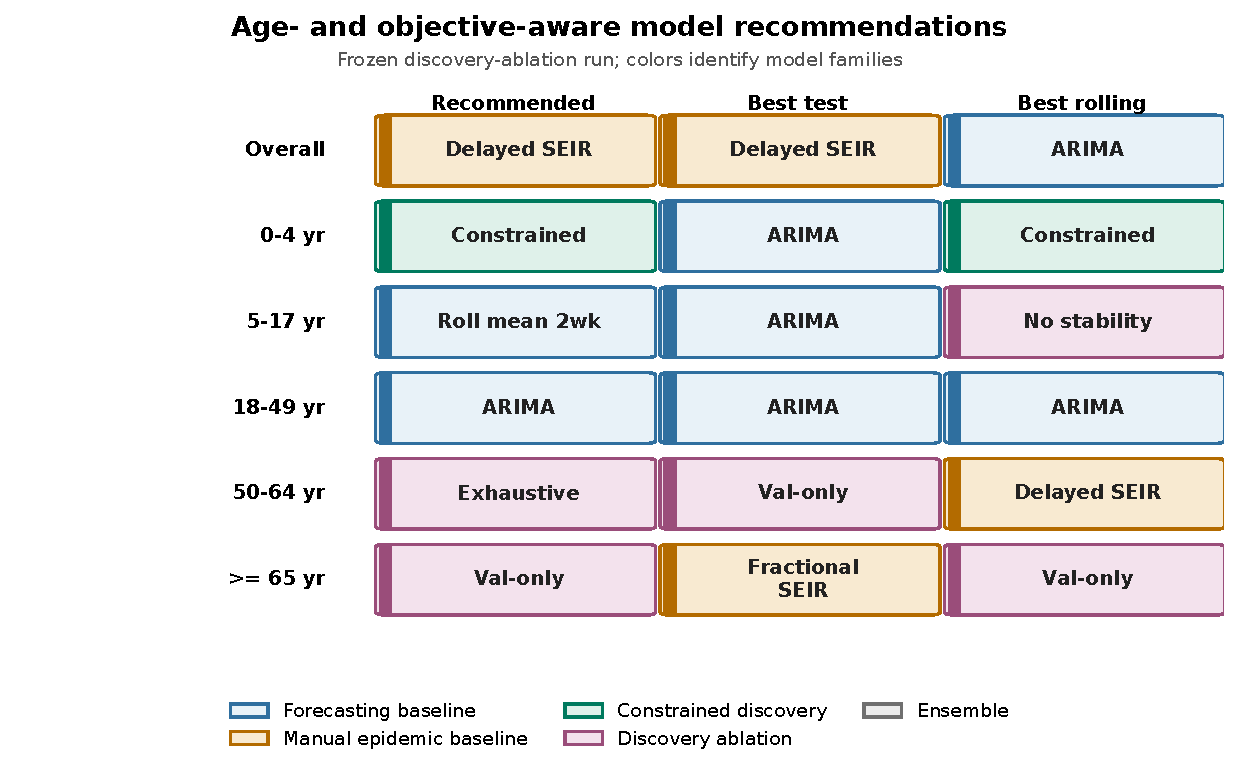
\includegraphics[width=\textwidth]{figures/fig1_recommendation_map.pdf}
\caption{Age- and objective-aware model recommendations from the frozen
discovery-ablation run. Different age strata favor different model families
and different evaluation objectives. The figure supports objective-aware
recommendation rather than a single global winner claim.}
\label{fig:recommendation-map}
\end{figure}

\begin{table}[H]
\centering
\small
\caption{Frozen recommendation summary from the discovery-ablation run. The
recommended model is the benchmark policy output, not a claim of universal
dominance.}
\label{tab:frozen-recommendations}
\begin{tabularx}{\textwidth}{>{\raggedright\arraybackslash}p{1.35cm}
>{\raggedright\arraybackslash}p{3.1cm}
>{\raggedright\arraybackslash}p{2.25cm}
>{\raggedright\arraybackslash}p{2.8cm}
>{\raggedright\arraybackslash}p{2.8cm}
X}
\toprule
Series & Recommended model & Decision type & Best test model & Best rolling model & Selected discovery structure \\
\midrule
Overall & \texttt{delayed\_observation\_seir} & test preferred &
\texttt{delayed\_observation\_seir} & \texttt{arima\_auto\_small} & -- \\
\texttt{0-4 yr} & \texttt{constrained\_structure\_discovery} &
stability preferred & \texttt{arima\_auto\_small} &
\texttt{constrained\_structure\_discovery} &
\texttt{SEIRS}, \texttt{delayed\_I}, delay 1 \\
\texttt{5-17 yr} & \texttt{rolling\_mean\_2wk} & balanced tradeoff &
\texttt{arima\_auto\_small} & \texttt{no\_stability\_discovery} & -- \\
\texttt{18-49 yr} & \texttt{arima\_auto\_small} & consensus &
\texttt{arima\_auto\_small} & \texttt{arima\_auto\_small} & -- \\
\texttt{50-64 yr} & \texttt{exhaustive\_structure\_discovery} &
balanced tradeoff & \texttt{validation\_only\_structure\_selection} &
\texttt{delayed\_observation\_seir} & \texttt{SIR}, \texttt{I}, delay 0 \\
\texttt{>= 65 yr} & \texttt{validation\_only\_structure\_selection} &
stability preferred & \texttt{fractional\_seir} &
\texttt{validation\_only\_structure\_selection} &
\texttt{SEIRS}, \texttt{I}, delay 0 \\
\bottomrule
\end{tabularx}
\end{table}

The clearest positive observation-aware discovery result is the pediatric
\texttt{0-4 yr} series. The benchmark recommends
\texttt{constrained\_structure\_discovery} as the stability-preferred model,
and the rolling-origin winner is also constrained discovery. The selected
structure is \texttt{SEIRS} with delayed infectious observation
\texttt{delayed\_I} and delay 1. Against the observation-fixed ablation,
constrained discovery reduces rolling absolute error by \num{0.0564} on
average for \texttt{0-4 yr}, with a bootstrap 95\% confidence interval from
\num{0.0173} to \num{0.1082}.

\begin{figure}[H]
\centering
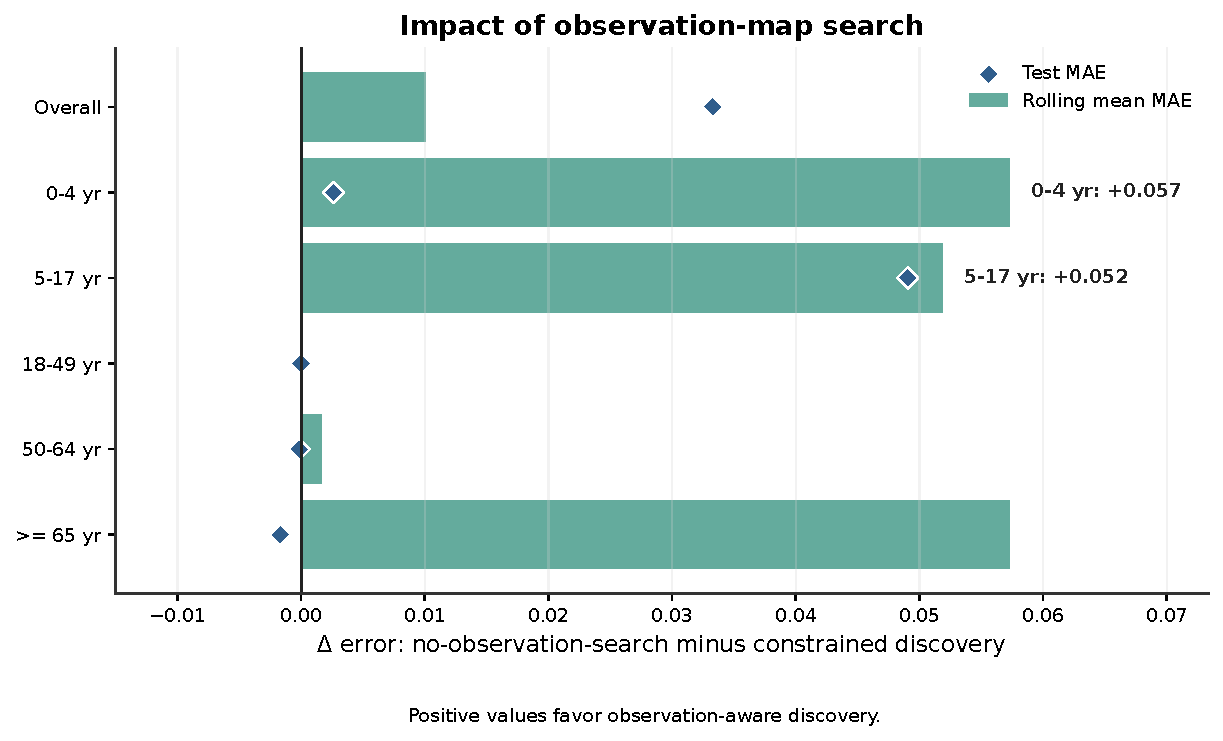
\includegraphics[width=0.98\textwidth]{figures/fig2_observation_search_impact.pdf}
\caption{Impact of observation-map search. Positive values mean that the
observation-fixed ablation has higher error than constrained discovery. The
clearest positive signal is in pediatric strata, especially \texttt{0-4 yr}.}
\label{fig:observation-search-impact}
\end{figure}

\begin{table}[H]
\centering
\small
\caption{Impact of disabling observation-map search. Positive deltas favor
constrained discovery. The \texttt{>= 65 yr} discovery rows include numerical
failure flags and should be interpreted descriptively rather than as positive
evidence.}
\label{tab:observation-search-impact}
\begin{tabular}{lcccc}
\toprule
Series & $\Delta$ test MAE & $\Delta$ rolling MAE & Constrained obs. & Fixed obs. \\
\midrule
Overall & \num{0.0333} & \num{0.0100} & \texttt{I} & \texttt{I} \\
\texttt{0-4 yr} & \num{0.0026} & \num{0.0573} & \texttt{delayed\_I} & \texttt{I} \\
\texttt{5-17 yr} & \num{0.0491} & \num{0.0519} & \texttt{delayed\_I} & \texttt{I} \\
\texttt{18-49 yr} & \num{-0.0000} & \num{-0.0000} & \texttt{I} & \texttt{I} \\
\texttt{50-64 yr} & \num{-0.0002} & \num{0.0017} & \texttt{I} & \texttt{I} \\
\texttt{>= 65 yr} & \num{-0.0017} & \num{0.0573} & \texttt{I} & \texttt{I} \\
\bottomrule
\end{tabular}
\end{table}

Adult strata are important negative evidence against overclaiming. The
\texttt{18-49 yr} series is best served by \texttt{arima\_auto\_small} in
both the held-out test split and rolling-origin evaluation. In paired
rolling-origin comparison, \texttt{arima\_auto\_small} has lower rolling
absolute error than constrained discovery for \texttt{18-49 yr}, with mean
difference \num{-0.0487} and a 95\% interval from \num{-0.0641} to
\num{-0.0323}. The \texttt{Overall}, \texttt{50-64 yr}, and
\texttt{>= 65 yr} strata also illustrate objective dependence: fixed test and
rolling-origin winners do not always agree.

\begin{figure}[H]
\centering
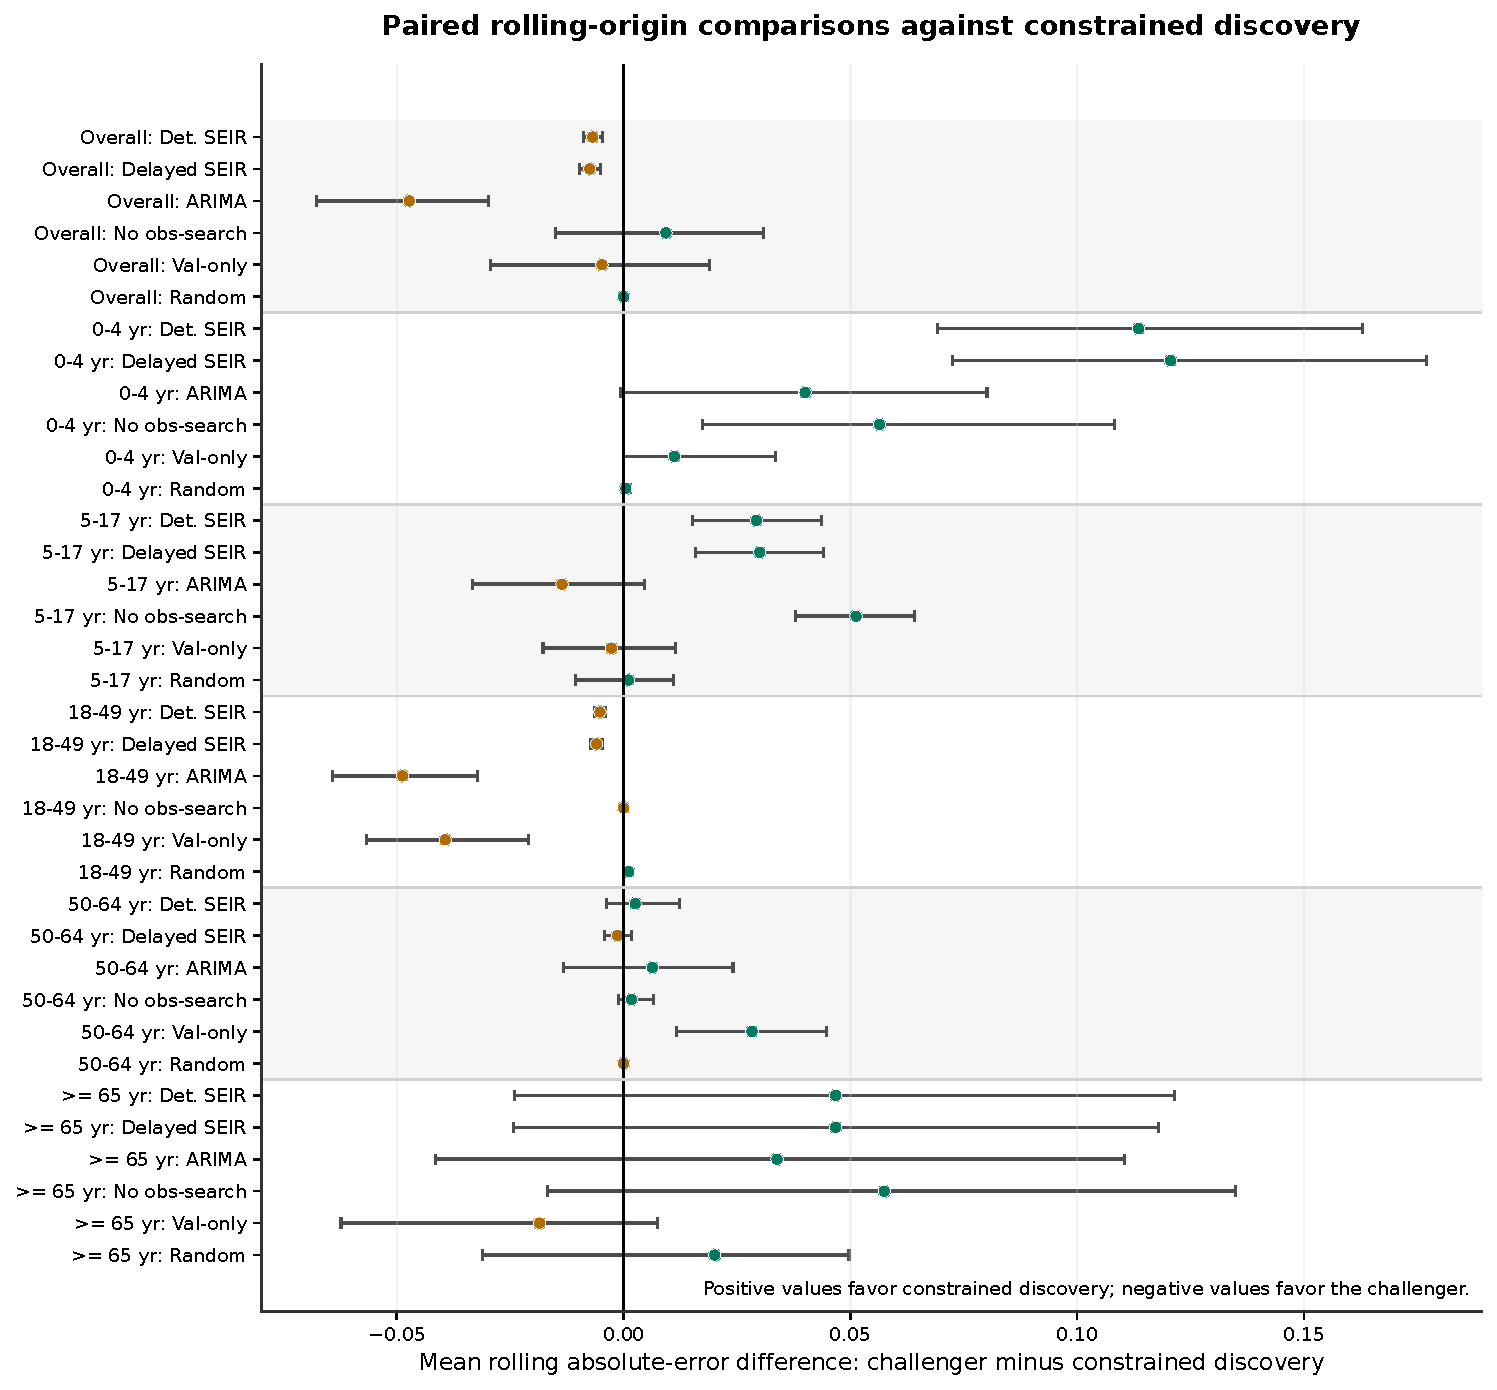
\includegraphics[width=\textwidth]{figures/fig4_paired_rolling_forest.pdf}
\caption{Post-hoc paired rolling-origin comparisons against constrained
discovery. Positive values favor constrained discovery; negative values favor
the challenger. These comparisons summarize evidence after model selection
and are not used for model selection.}
\label{fig:paired-rolling-forest}
\end{figure}

Finally, the compact multi-season appendix evaluates six completed
FluSurv-NET seasons as independent within-season trajectories. Its pediatric
results are mixed across seasons: the \texttt{0-4 yr} observation-aware signal
from the frozen benchmark is not uniformly repeated under the reduced
robustness budget. We therefore treat the frozen discovery-ablation benchmark
as the clearest evidence for the \texttt{0-4 yr} delayed-observation finding
and use the multi-season check as a robustness caveat rather than as a
stronger global claim.

The frozen summary retains numerical diagnostics for every model-series row.
There are 11 flagged rows among 108 model-series evaluations. These rows are
retained for transparency but are not used to support positive claims,
especially for interpretations involving the flagged \texttt{>= 65 yr}
constrained-discovery row.
